\documentclass{article}
\usepackage[utf8]{inputenc}
\usepackage[T1]{fontenc}


% Language setting
% Replace `english' with e.g. `spanish' to change the document language
\usepackage[french]{babel}

% Set page size and margins
% Replace `letterpaper' with `a4paper' for UK/EU standard size
\usepackage[letterpaper,top=2cm,bottom=2cm,left=3cm,right=3cm,marginparwidth=1.75cm]{geometry}

% Useful packages
\usepackage{amsmath}
\usepackage{graphicx}
\usepackage[colorlinks=true, allcolors=blue]{hyperref}
\usepackage{pgfgantt}
\usepackage[margin=1in]{geometry}
\usepackage{pdflscape} % ou lscape
\usepackage{tikz-uml}

\usepackage{fancyhdr}

\begin{document}

\section{Classes}

\subsection{Classe Enemy}
\paragraph{}
La classe Enemy représente les ennemis dans le jeu. Elle gère les attributs tels que la santé, la vitesse, et la position. Elle inclut également des méthodes pour déplacer les ennemis le long du chemin défini par l'algorithme de "chemin le plus court".

Elle contient une structure "enemy" qui regroupes les informations décrivant un ennemi (nom, forme (shape), position, vie, vitesse, carapace, attaque, vitesse d'attaque, portée, pathPoints, currentPathIndex, nombre d'ennemis).


"pathPoints" est un vecteur de sf::Vector2f qui contient les points du chemin que l'ennemi doit suivre. "currentPathIndex" est un entier qui indique l'index actuel dans le vecteur pathPoints.


Spawn Position() : Cette méthode initialise la position de l'ennemi sur la carte de manière aléatoire.

Move() : Cette méthode déplace l'ennemi le long du chemin défini par les points dans pathPoints. Elle utilise la vitesse de l'ennemi pour déterminer la distance à parcourir à chaque mise à jour.
Grâce à la boucle "while", la fonction move() est exécutée en continue. Ainsi SolveAStar() est appelé régulièrement pour recalculer le chemin de l'ennemi en fonction de sa position actuelle.


Draw() : Cette méthode dessine l'ennemi à sa position actuelle sur la fenêtre de jeu.


Pour contenir les caractéristiques et le chemin de chaque ennemi, un vecteur "groupe\_enemies" est utilisé. Chaque élément du vecteur est une instance de la structure "enemy".


\subsection{Classe Tower}
\paragraph{}

La classe Tower représente les tours que le joueur peut placer sur la carte. Elle gère les attributs tels que le type de tour, les dégâts, la portée, et le coût. Elle inclut des méthodes pour attaquer les ennemis lorsqu'ils entrent dans sa portée.


\subsection{Classe Pathfinding AStar}
\paragraph{}

Afin de permettre aux ennemis de se déplacer de manière intelligente sur la carte, un algorithme de pathfinding est nécessaire.
Dans un premier temps, une lecture de la description de la librairie boost_graph a permis de cerner les algorithmes de pathfinding disponibles.

lien de descriptionn: \url{https://www.boost.org/doc/libs/latest/libs/graph/doc/index.html}

L'algoritme Dijkstra's Shortest Paths a été envisagé. Mais après réflexion et comparaison sur wikipédia, l'algorithme A* (A-star) a été préféré car il est généralement plus efficace pour les jeux vidéo et les applications en temps réel.


La classe Pathfinding AStar implémente l'algorithme A* pour trouver le chemin le plus court entre deux points sur la carte.
Elle est utilisée par la classe Enemy pour déterminer le chemin à suivre.


Tout d'abord, le programme de A* est inspiré du github suivant : 


\url{https://github.com/OneLoneCoder/Javidx9/blob/master/ConsoleGameEngine/SmallerProjects/OneLoneCoder_PathFinding_AStar.cpp}


La vidéo suivante explique le fonctionnement de l'algorithme A* : 


\url{https://www.youtube.com/watch?v=icZj67PTFhc} 


Après modification du code source pour une utilisation avec SFML, l'algorithme A* fonctionne de la manière suivante :
\begin{itemize}


    \item La carte est représentée comme une grille de nœuds, où chaque nœud correspond à une cellule de la carte. 
    Chaque nœud a des attributs tels que son état (libre ou occupé), ses coordonnées, 
    le coût pour atteindre ce nœud depuis le nœud de départ, le coût estimé pour atteindre le nœud d'arrivée depuis ce nœud, 
    un vecteur contenant ses voisins, et un pointeur qui sera dirigé vers son noeud parent.


    \item CreateNodes() : Cette méthode initialise la grille de nœuds en fonction de la carte du jeu. 
    Elle créé des nœuds pour chaque cellule de la carte et définit leurs attributs initiaux.
    

    \item EnemyNode() : Cette méthode traduit la position actuelle de l'ennemi en coordonnées de nœud dans la grille.
    Elle n'est pas forcément située au centre d'un nœud.


    \item SolveAStar() : C'est la méthode principale qui implémente l'algorithme A*. Elle prend en entrée les coordonnées de l'ennemi,
    et retourne un vecteur de nœuds représentant le chemin le plus court trouvé.
    

    \item Draw() : Cette méthode est utilisée pour visualiser la grille de nœuds et le chemin trouvé.
    Elle dessine chaque nœud avec une couleur différente en fonction de son état, et trace le chemin en reliant les nœuds du chemin trouvé.


\end{itemize}

Le résultat obtenu après l'exécution de l'algorithme A* est figuré ci-dessous :

\begin{figure}[!h]
\centering
    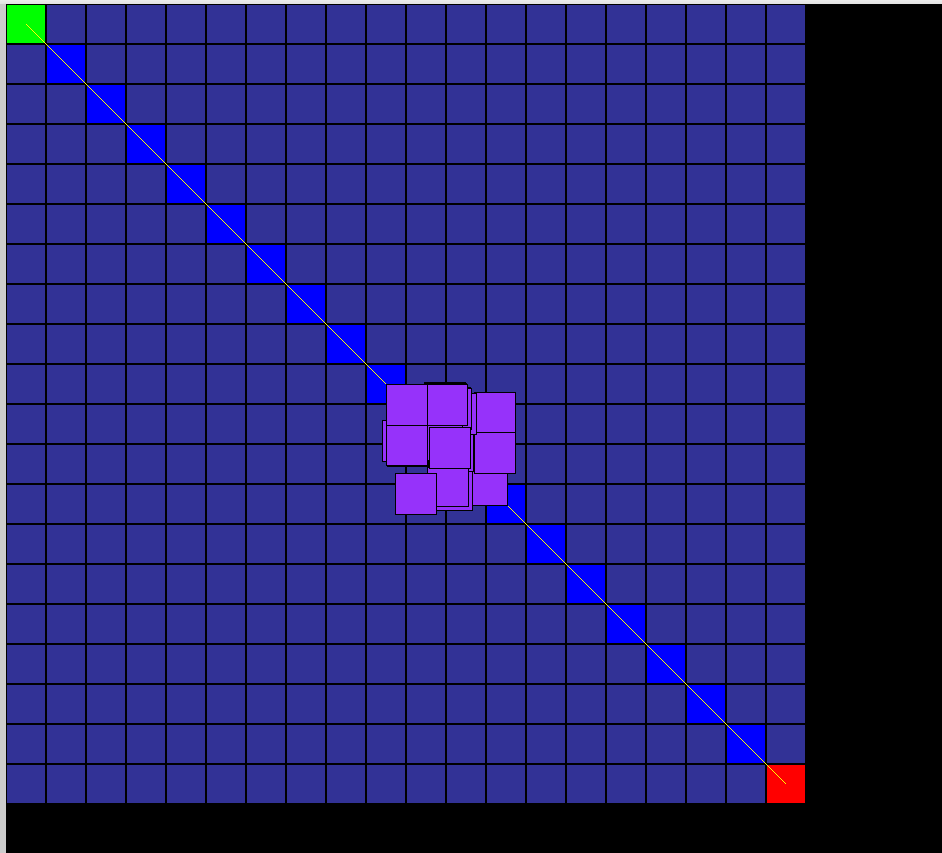
\includegraphics[width=1\textwidth]{figs/ASTAR.png}
    \caption{Déplacement des ennemis avec l'algorithme A*}
\end{figure}

\paragraph{}

Le chemin le plus court est représenté par une ligne jaune reliant les nœuds verts (noeud de départ) et rouge (nœud d'arrivée).
Les nœuds bleus claires représentent les nœuds libres visités par l'algorithme, tandis que les nœuds bleus foncés représentent les nœuds libres non visités.


Ici, seulement un noeud est vert, car on affiche le noeud de départ du premier ennemi apparu.


\section{Difficulés rencontrées}
\paragraph{}
Les principales difficultés rencontrées à ce stadde du projet ont été les suivantes :


\item La mise en place de l'algorithme A* pour le pathfinding des ennemis. Cela a nécessité une compréhension approfondie de l'algorithme et son adaptation à la librairie SFML.
\item l'échange de données entre les différentes classes, notamment entre la classe Enemy et la classe Pathfinding AStar.
\item la définition et la gestion du movement fluide des ennemis le long du chemin calculé par l'algorithme A*.

Important : Après plusieurs tentatives de résolution, ChatGPT a été utilisé pour résoudre certaines erreurs de compilation mais aussi pour surmonter les difficultés lors de la création de A* et du mouvement des ennemis.

\section{Pistes d'amélioration}
\paragraph{}

La structure des ennemis peut être remplacée par des classes dérivées pour chaque type d'ennemi. Cela permettrait une meilleure organisation du code et une plus grande flexibilité pour ajouter de nouveaux types d'ennemis avec des comportements spécifiques.


La création de tours devra être implémentée, avec des classes dérivées pour chaque type de tour. Chaque classe de tour pourrait avoir des attributs et des méthodes spécifiques, comme le type de dégâts infligés, la portée, et la vitesse d'attaque.


A* devra prendre en compte les tours placées par le joueur pour recalculer le chemin des ennemis en temps réel. Cela ajouterait une dimension stratégique au jeu, car les joueurs pourraient influencer le chemin des ennemis en plaçant des tours de manière stratégique.

De plus, au lieu de prendre en compte qu'un seul noeud de fin, A* pourrait être modifié pour prendre en compte plusieurs noeuds de fin, représentant plusieurs points d'arrivée possibles pour les ennemis.

Cela permettrait aux ennemis de choisir le chemin le plus court vers n'importe quel point d'arrivée.

\newpage

\end{document}